%\documentclass[a4paper,10pt]{article}
\documentclass[conference]{format/IEEEtran}
%\usepackage[utf8x]{inputenc}
\usepackage[utf8]{inputenc}
\usepackage{graphicx}

%opening
\title{Automatic Detection of Bad Programming Habits in Scratch: A Preliminary Study}
%\author{Jesús Moreno, Gregorio Robles}

\author{\IEEEauthorblockN{Jesús Moreno}
\IEEEauthorblockA{INTEF \& Programamos.es\\
Madrid, Spain\\
jesus.moreno@programamos.es}
\and
\IEEEauthorblockN{Gregorio Robles}
\IEEEauthorblockA{GSyC/LibreSoft\\Universidad Rey Juan Carlos\\
Madrid, Spain\\
grex@gsyc.urjc.es}}


\begin{document}

\maketitle

\begin{abstract}
%This paper describes a method for automatic detection of two bad programming habits that students learning to program with Scratch incur, such as the repetition of code and object naming, and raises ideas to try to avoid such situations. FIXME: some methodology, results and conclusions should be included in the abstract.
Using Scratch as a tool to teach Computer Science or develop Computational Thinking from other disciplines is increasingly common in all levels of education, and it is possible to find well-documented success case studies from primary school to university experiences.

However, there are reports indicating that students learning to program in this environment show certain habits that are contrary to the basic programming recommendations. In our work as instructors with high school students learning to program with Scratch, we also detected some common bad practices, such as the repetition of code and object naming, and this study focuses on checking whether these issues can be found in the projects shared on the community website. 

To test this hypothesys, we downloaded 100 projects from the Scratch website and analyzed them with two plug-ins we developed to automatically detect these bad practices. The plug-ins extend the functionality of the tool Hairball, a static code analyzer for Scratch projects. The obtained results indicate that, in general, projects in the repository also incur in the investigated malpractices.

Along with suggestions for future work, some ideas that might assist to avoid such situations are proposed in the conclusions of the paper.

\end{abstract}

\section{Introduction}

Scratch~\cite{resnick2009scratch}  is a programming environment including a visual programming language designed for children over 6 years old, a development environment and a website where the community can host their projects, run, study and reuse other programs, and share ideas or suggestions with other programmers. Although there are several similar visual programming languages, Scratch is undoubtedly the most successful one with more than three million registered users on its website and more than five million shared projects in its repository\footnote{See http://scratch.mit.edu/statistics/}.

Scratch is being used both in extracurricular activities~\cite{kafai2010entering} or summer camps~\cite{adams2010scratching}, as in elementary schools~\cite{wilson2012evaluation}, high schools~\cite{meerbaum2013learning} and even universities worldwide~\cite{malan2007scratch}. Its capacity to bring computer programming to children and teenagers with the aim of fostering computational thinking abilities and to promote ICT studies, and its success to teach both basic and advanced programming concepts (concepts such as user interaction, conditional statements, communication and synchronization, logical expressions and data representation are taught) has been documented~\cite{maloney2008programming, franklin2013assessment, wolz2009starting}.

However, it is also possible to find studies that have detected some bad programming habits in students learning to program in this environment~\cite{meerbaum2011habits}. In this line, in our work as instructors we have detected bad habits despite having insisted our students to avoid them. As these habits are contrary to the basic programming recommendations, our study tries to find out if they are also common in the projects shared in the Scratch repository, and propose some ideas to try to avoid such situations.

FIXME: the goal of this paper is to... 
% ¿No estaría explicado justo en el párrafo de encima? ¿Habría que explicarlo más detalladamente?

The structure of this paper is as follows: In section~\ref{sec:background} a brief overview of Scratch is presented, including some research studies that have investigated learning in this environment and other studies that automate the evaluation of learning. In section~\ref{sec:methodology} our work methodology is briefly described. Section~\ref{sec:findings} presents the results we have obtained from applying our methodology on a small sample of Scratch projects. Finally, Section~\ref{sec:conclusions} contains the conclusions of our study and some ideas and suggestions for future work are discussed.

\section{Background}
\label{sec:background}

Scratch is a visual programming environment, developed by the Lifelong Kindergarten group at the MIT Media Laboratory, that allows to program interactive projects using a drag-and-drop approach with different pieces or \textit {Lego} style blocks~\cite{resnick2009scratch}. Scratch was designed with the main goal of encouraging young people to program, and most of its users are novice learners with no prior programming experience~\cite{maloney2010scratch}. The environment is designed to encourage users to manipulate and modify various media types, so that children and teenagers can create projects that they find interesting and attractive, such as animated stories, games or interactive presentations~\cite{maloney2008programming}.

Scratch also offers a website where the projects programmed by the community are published. The code of programs hosted there can be studied and analyzed, and it is possible to make suggestions and reuse the code, so there are lots of valuable resources available for anyone willing to start to program. This approach also offers the opportunity to learn certain social skills related to programming, such as sharing and contributing to the community~\cite{scaffidi2012skill}.

% repe
%There are many papers showing that Scratch works as a tool for learning to program~\cite{maloney2008programming, franklin2013assessment, scaffidi2012skill, malan2007scratch}, and there are success stories at different educational levels, environments and disciplines showing that students learn concepts such as user interaction, conditional statements, communication and synchronization, logical expressions and data representation.

Despite the positive impact of Scratch, Meerbaum-Salant, Armoni and Ben-Ari~\cite{meerbaum2011habits} prove that students learning to program in this environment show some bad habits that are contrary to recommended programming practices. In particular, they show a tendency to excessive decomposition and a bottom-up development process, starting with individual blocks of Scratch.

Aiming to simplify the process of evaluating computational thinking and help evaluators with an automatic tool, Hairball was created~\cite{boe2013hairball}. Hairball is a static analyzer of Scratch projects inspired by Lint\footnote{http://www.unix.com/man-page/FreeBSD/1/lint} that tries to detect programming errors in Scratch projects, such as not initializing the value of a variable or the state of a character, sending messages that are not received by any program, including code that is never run, among others.

\section{Methodology}
\label{sec:methodology}

In our work as instructors with high school students, we found that, despite our constant insistence and warnings to try to avoid them, many students show two bad habits in a regular basis that have to do with object naming and code repetition.
    
On the one hand, it is very common that students do not change the names of the characters, which are automatically named by the environment as \textit{SpriteX}, where X is an incremental number. When the amount of characters in a project increases, it is quite hard to know which object relates to a given statement, contributing to poor code readability, slowing the project programming and complicating debugging to fix bugs.

On the other hand, it is also very common to see students repeating code in the same project, sometimes even in the same character programs. Thus, besides complicating the maintenance and updating of the code, abstraction and modularization, two key components of the development of computational thinking~\cite{wing2008computational}, are not trained.

In order to detect these two behaviors in Scratch projects, we have developed two plug-ins for the Hairball environment~\cite{boe2013hairball}, which in turn makes use of \textit{kurt}\footnote{https://github.com/blob8108/kurt}, a library implemented in python, to automate the detection of this type of bad practices in programs developed in this environment.

The plug-in \textit{convention.SpriteNaming}\footnote{https://github.com/jemole/hairball/blob/master/hairball/plugins/convention.py} analyzes a Scratch project to check if the names of its characters begin with the string \textit{Sprite}, which indicates that the user has not changed its name and has left the one the system assigns by default to every new character added to the project.

The plug-in \textit{duplicate.DuplicateScripts}\footnote{https://github.com/jemole/hairball/blob/master/hairball/plugins/duplicate.py} analyzes a Scratch project to try to locate repeated complete programs within a project. In order to do so the plug-in runs each project and gets the \textit{tokens} of the different blocks of the programs, so that two blocks that only differ in the values they receive are considered to be equal. To illustrate the operation of this plug-in, picture \ref{fig:CodeRepetition1} shows two scripts containing the same blocks with the only difference of the values received by parameter.
\begin{figure}
  \centering
    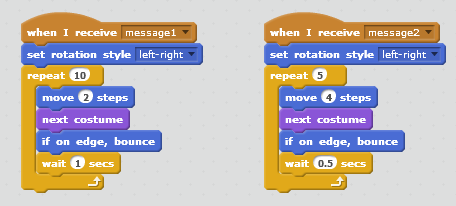
\includegraphics[width=9cm]{img/CodeRepetition1.png}
  \caption{Two scripts repeating code}
  \label{fig:CodeRepetition1}
\end{figure}


When these scripts are analyzed by the plug-in and are translated into \textit{tokens} they would be considered equal, as their code would be translated to the next set of \textit{tokens}:
\begin{verbatim}
 'set rotation style %s'
 'repeat %s%s'
 'move %s steps'
 'next costume'
 'if on edge, bounce'
 'wait %s secs'
\end{verbatim}

Thus, the correct way to implement this project would have been as shown in Figure \ref{fig:CodeRepetition2}, defining a new set of blocks that receives several values per parameter and reusing the block created in both programs. This solution would involve improvements regarding maintenance, updating and debugging.

\begin{figure}
  \centering
    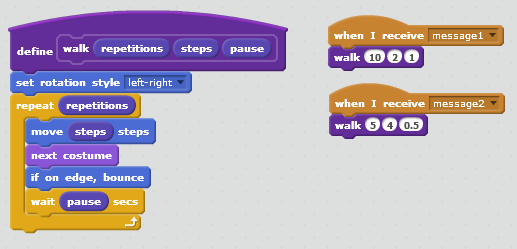
\includegraphics[width=9cm]{img/CodeRepetition2.png}
  \caption{Defining own blocks to avoid code repetition}
  \label{fig:CodeRepetition2}
\end{figure}


In order to test the functionality of the developed plug-ins and check whether these behaviors that we detected in our work are also common in the projects of the Scratch repository, we proceeded to download 100 projects from the repository. As the possibility for users to define their own blocks, using \textit{def\_block} feature, is only available since the release of Scratch 2.0, we selected and downloaded projects created after that date.


\section{Findings}
\label{sec:findings}

Data obtained after analyzing 100 downloaded projects confirm that observations made with our students are also very common in the community projects.

Regarding the lack of habit of renaming the characters and not using the default name assigned by the environment, the 79\% of the analyzed projects contained at least one \textit{SpriteX} character not renamed.

As an example to illustrate the drawbacks associated with this malpractice, picture \ref{fig:SpriteNaming} shows a script that is difficult to read as the character area must be explored to find which character refers to a particular block, making the program difficult to debug any problems should arise, making it hard to code improvements and even slowing down the programming time, as the name of the character must be memorized or checked every time a block is added. 

\begin{figure}
  \centering
    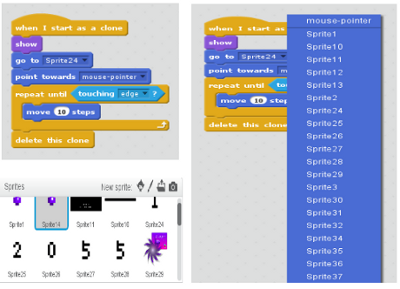
\includegraphics[width=9cm]{img/SpriteNaming.png}
  \caption{Sprites with default names}
  \label{fig:SpriteNaming}
\end{figure}

As for the repetition code, 62\% of the analyzed projects contained at least one repeated program. In fact, only 17\% of the analyzed projects made use of block \textit{def\_block} to define its own blocks that can be reused in other parts of the project. 

\section{Conclusions and further research}
\label{sec:conclusions}

%FIXME: In this paper... short summary of what we have done and why

This paper shows the preliminary results of a study regarding two bad programming habits we have detected in our work as instructors with high school students learning to program with Scratch. In order to check if these bad habits, which have to do with object naming and code repetition, are also commonly found in the projects shared in the community repository, we downloaded 100 proyects and analyzed them with two plug-ins we developed for Hairball, detecting that most of the inspected proyects, 79\% and 62\%  respectively, fell into these issues.

Regarding the object naming, it is curious that Scratch users name correctly, i.e., semantically meaningful, the variables used in their projects. In our opinion the reason to explain this paradox is because it is mandatory to assign a name to a variable the moment it is created, as the environment does not name it by default. However, when creating a new character a  \textit{SpriteX} name is assigned automatically. In our views, a change of this feature of the environment, forcing users to name new objects, might eliminate this bad practice.

Regarding the code repetition and the low usage Scratch users make of the possibility of creating their own blocks (the equivalent of defining methods or procedures in other languages), works as the one performed by Seiter and Foreman~\cite {seiter2013modeling}, in which they show that abstraction and modularization capacities are concepts that seem to be developed from a certain age, may explain the low rates of use of this functionality, since a significant part of the Scratch community consists of children under 10 years old\footnote{http://scratch.mit.edu/statistics/\#age}. Future studies should further investigate to continue advancing in the definition of an appropriate framework for different ages, as well as to check whether users learning online and those who do it in a regulated environment show different use rates of this functionality.

%In the near future, we plan to... FIXME... talk about next steps: i) more analysis, ii) more projects, iii) web-based tool that provides learning-oriented feedback in an automatic way.

In the near future we plan to extend the scope of our study developing new plug-ins to automate the detection of other issues, such as the degree of development of computational thinking demonstrated in a project, and analyzing a much larger number of projects to achieve more accurate conclusions. In this sense, the release of a research dataset with the first five years of data from the Scratch repository\footnote{https://sites.google.com/site/scratchdatameeting/} will be certainly a great help to our work. Finally, we are in the process of developing a website that will allow students to receive feedback from each of its programs with warnings of potential errors and tips to improve their code, and will offer teachers a tool to assist them in correcting their students proyects.

\section*{Acknowledgments}

The work of Gregorio Robles has
been funded in part by the Spanish Government under project 
SobreSale (TIN2011-28110) and by the Comunidad de Madrid 
under project eMadrid (FIXME). 

\bibliographystyle{abbrv}
\bibliography{scratch}
\end{document}
